\section{Implementação}
\label{sec:implementacao}

Para a implementação desse trabalho, foi definida a gramática simples que
opera apenas sobre inteiros. Não ha ativação de funções e apenas um escopo
(global). Na Listagem \ref{lst:fib}, temos um programa-exemplo para o cálculo
da sequência de Fibonacci.

\lstinputlisting[label=lst:fib,caption=Exemplo de Cálculo
da Sequência de Fibonacci]{compiler-src/examples/fibonacci/fibonacci.lang}

Verificamos no exemplo da Listagem \ref{lst:fib}, que a linguagem suporta
construções comumente vistas numa linguagem de programação mais
sofisticada. Temos uma série de atribuições, leitura da entrada-padrão,
estrutura condicional (\emph{se-senão}), estrutura de laço (\emph{enquanto})
e escrita para a saída-padrão. Entretanto não há suporte para vetores
(\emph{arrays}), números de ponto flutuante e cadeias de caracteres
(\emph{strings}), recursos presentes nas linguagens de programação reais.

Mesmo na ausência destes recursos, nossa linguagem possibilita o estudo da
implementação e funcionamento de um compilador. A definição formal da
linguagem encontra-se na Listagem \ref{lst:grammar}.

\begin{lstlisting}[label=lst:grammar,caption=Gramática reconhecida]
  program : stmts
          ;

  stmts : stmts stmt
        | stmt
        ;

  stmt  : if_decl SEMI
        | while_decl SEMI
        | attrib_decl SEMI
        | read_decl SEMI
        | write_decl SEMI
        ;

  if_decl  : IF LPAREN bool RPAREN stmts END
           | IF LPAREN bool RPAREN stmts ELSE stmts END
           ;

  while_decl : WHILE LPAREN bool RPAREN stmts END
             ;

  attrib_decl : ID ATTR expr
              ;

  read_decl : READ ID
            ;

  write_decl : WRITE ID
             ;

  expr : expr PLUS expr
       | expr MINUS expr
       | expr TIMES expr
       | expr OVER expr
       | factor
       | bool
       ;
  bool : expr OR expr
       | expr AND expr
       | expr EQ expr
       | expr NEQ expr
       | expr GT expr
       | expr LT expr
       | expr GE expr
       | expr LE expr
       | expr
       ;

  factor : LPAREN expr RPAREN
         | ID
         | NUM
         ;
\end{lstlisting}

Como podemos perceber um programa é um conjunto de instruções delimitados por
ponto-e-vírgula. A linguagem disponibiliza uma instrução para execução
condicional e uma outra para laços de repetição. Ambas tomam como parâmetro
uma expressão que possa ser avalidada como um inteiro. Como ocorre na
\emph{Linguagem C} uma expressão cujo valor seja avaliado como 0 (zero) é
considerada \emph{falsa} e qualquer outro valor é avaliado como
\emph{verdadeiro}.

Adicionalmente as instruções de laço e condicionais, a linguagem propicia uma
instrução para o armazenamento da avaliação de uma expressão (atribuição de
variável) e duas instruções de Entrada e Saída. A instrução de entrada-padrão
(\emph{leia}) lê um inteiro do teclado e a instrução de saída (\emph{escreva})
escreve o valor atribuído a uma variável na saída-padrão (possivelmente um
terminal).

As operações relacionais (booleanas) possuem prioridades conforme a Tabela
\ref{tab:prioridades}, sendo que as operações que aparecem primeiro, na
tabela, possuem maior prioridade. As operações matemáticas possuem a
precedência usual.

\begin{table}
	\begin{center}
		\begin{tabular}{c l}
			< <= > >= & Menor, Menor ou igual, Maior, Maior ou igual \\
			== !=      & Igualdade,  Desigualdade \\
		\end{tabular}
	\end{center}
	\caption{Prioridades dos Operadores Relacionais}
	\label{tab:prioridades}
\end{table}

A gramática da Listagem \ref{lst:grammar} é ambígua (verificar Seção
\ref{sec:ambig}), todavia as ambiguidades são resolvida pelas prioridades já
discutidas, durante o processo de análise sintática.

Para a implementação do compilador foi escolhida a \emph{linguagem C}. A
escolha foi baseada na familiaridade do autor com a linguagem, além da farta
disponibilidade de ferramentas e literatura sobre a referida linguagem. Mais
informações podem ser obtidas em \citeonline{c-book}, \citeonline{KeR} e
\citeonline{schildt}

\begin{figure}[htb]
	\centering
	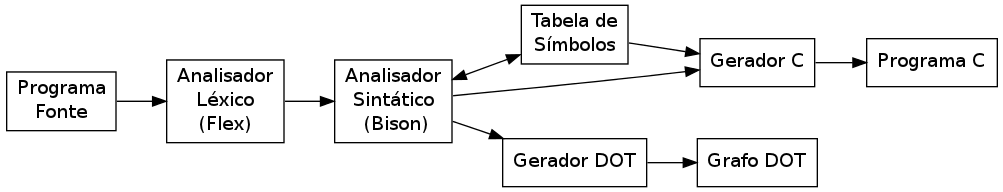
\includegraphics[scale=0.43]{compiling_schema}
	\caption{Módulos do Compilador}
	\label{fig:compiler_schema}
\end{figure}

A Figura \ref{fig:compiler_schema} demonstra o esquema de interação entre
os módulos do compilador. O programa-fonte é lido pelo \emph{Analisador
Léxico} que produz o \emph{fluxo de tokens} que alimenta o \emph{Analisador
Sintático}. Este verifica se os tokens recebidos são corretos para a
\emph{gramática} determinada, produz a \emph{Árvore Sintática} e insere e
consulta entradas na \emph{Tabela de Símbolos}. O \emph{Gerador C} navega
na \emph{Árvore Sintática} para gerar as construções correspondentes
em C, consultando a \emph{Tabela de Símbolos} quando necessário.
O \emph{Gerador DOT} monta a representação gráfica apenas com as
informações disponibilizadas pela \emph{Árvore Sintática}. Por fim,
compilamos o programa C gerado, com um compilador C padrão, para obtermos
o programa executável e compilamos o arquivo DOT (\emph{Grafo DOT}) com o
aplicativo \textbf{dot} (Seção \ref{sec:impl_gen_dot}) para obtermos a
representação gráfica da lógica do programa-fonte.

\subsection{Estruturas de Dados}
As principais \emph{Estruturas de Dados} estão definidas na Listagem
\ref{global.h} (global.h). São definidos três enumeradores que serão
utilizados para diferenciar os nós da Árvore Sintática: \emph{node\_kind},
\emph{stmt\_kind} e \emph{expr\_kind}. O enumerador \emph{node\_kind}
especifica se determinado nó é uma \textbf{instrução} ou \textbf{expressão}.
Caso seja uma \textbf{instrução}, verificamos seu tipo no enumerador
\emph{stmt\_kind} que possui como valores possíveis: \emph{if\_k},
\emph{while\_k}, \emph{attrib\_k}, \emph{write\_k}, \emph{read\_k}, para as
instruções de escolha condicional, laço de repetição, atribuição de variável,
escrita e leitura, respectivamente. Caso seja o nó seja uma
\textbf{expressão}, verificamos o enumerador \emph{expr\_kind}, que nos
possibilita os valores seguintes: \emph{op\_k}, \emph{id\_k} e
\emph{const\_k}, para indicar expressões aritméticas e booleanas, a presença
de um identificador ou uma constante numérica, respectivamente.

Os \emph{tokens} para constantes numéricas e identificadores são armazenados
numa estrutura chamada \emph{token\_t}. A estrutura mantém a linha em que o token
foi encontrado e uma união que armazena um inteiro (constante numérica), ou um
ponteiro para uma cadeia de caracteres (identificadores). Para os demais
casos, apenas o tipo do token é retornado pelo analisador léxico.

A Árvore Sintática é produzida por nós da estrutura do tipo \emph{node\_t}. A
sequência de instruções é representada por uma lista ligada utilizando o
apontador \emph{next}. As instruções aninhadas (repetições e condicionais) são
representadas como nós filhos. Para os nós que representam expressões o
atributo da expressão é armazenado numa união conforme o tipo da expressão
(operação aritmética, um identificador, ou uma constante numérica).

\subsection{O Programa Principal}
O programa principal, \emph{compiler.c}, é bastante simples e está disponível
no Apêndice \ref{apx:listings} na Listagem \ref{compiler.c}.

Primeiramente são configuradas as variáveis de chaveamento, com base nas opções
passadas na linha de comando. Para isso são feitas sucessivas chamadas a
função \emph{getopt()}, presente na biblioteca-padrão da linguagem C.

São configuradas as variáveis que armazenam as referências para o arquivo de
entrada (que será utilizada pelo Analisador Léxico) e para a Tabela de
Símbolos (utilizada no Analisador Sintático). Em seguida, é chamada a função
que ativa o Analisador Sintático (\emph{yyparse()}).

Ativações adicionais como imprimir árvore sintática e tabela de símbolos,
gerar código C (Seção \ref{sec:gen_c}) e DOT (\ref{sec:gen_dot}), são feitas
conforme as opções passadas na linha de comando.


\subsection{Análise Sintática}
O Analisador Sintático foi produzido utilizado o código gerado pela ferramenta
\emph{GNU/Bison} \cite{bison}. \emph{Bison} é uma implementação do \emph{YACC}
(Yet Another Compiler Compiler {--} Um Outro Compilador de Compiladores), um
gerador de analisadores sintáticos ascendentes que recebe um arquivo de
especificações da gramática a ser reconhecida (descrito numa gramática livre
de contexto) e produz código C para cada regra sintática reconhecida.

O arquivo da especificação está listado no Apêndice \ref{apx:listings} na Listagem
\ref{parser.y}, arquivo parser.y. A especificação é dividida em 3 partes,
separadas pelos caracteres \emph{\%\%}. Na primeira, são incluídas o preâmbulo
e as declarações de configuração do \emph{Bison}. Na segunda, estão as regras
gramaticais e suas respectivas regras semânticas. Na terceira, inclui-se
quaisquer funções auxiliares que forem necessárias.

Na seção inicial da especificação, o código listado entre \emph{\%\{} e
\emph{\%\}} será incluído diretamente no arquivo gerado, em seguida é
definido, como uma união, o tipo de dados retornado pelo analisador gerado,
bem como a declaração dos tokens (que nesse contexto também são os símbolos
terminais da gramática) e as precedências das operações ambíguas.

As regras gramaticais, na segunda seção do arquivo de especificação, são
idênticas àquelas listadas no início deste capítulo (Seção
\ref{sec:implementacao}), acrescidas das ações semânticas equivalentes. O
exemplo da gramática para a instrução de escrita de um inteiro encontra-se
na Listagem \ref{lst:grammar_write_decl}. Este trecho de código indica que o
Analisador Sintático deve receber um token \textbf{WRITE} seguido de um token
\textbf{ID} do Analisador Léxico. Quando isso ocorrer é criado um novo nó de
\emph{instrução} do tipo \emph{escrita}, que será armazenado na
pseudo-variável \textbf{\$\$} para ser retornado e incluído na Árvore
Sintática. Também são armazenados no nó o nome do Identificador (variável) que
deverá ser escrita e a sua localização no arquivo-fonte.

\begin{lstlisting}[label=lst:grammar_write_decl,caption=Instrução de Escrita]
write_decl : WRITE ID
           {
            $$ = new_stmt_node(write_k);
            $$->child[0] = new_expr_node(id_k);
            $$->child[0]->attr.name = copy_str ((yylval.token)->value.name);
            $$->lineno = yylval.token->lineno;
           }
           ;
\end{lstlisting}

As demais regras são bastantes parecidas com aquela demonstrada na Listagem
\ref{lst:grammar_write_decl}, exceto pela regra que define a atribuição de uma
variável. Para as atribuições (verificar Listagem \ref{lst:grammar_attr_decl})
é necessário declarar uma regra implícita para armazenarmos os valores do token
\textbf{ID} antes de construirmos o nó correspondente. Isso é necessário, pois
o Analisador Sintático só sabe que se trata de uma instrução de atribuição
depois de reconhecer o não-terminal \emph{expr}. Quando \emph{expr} é
reconhecido as referências para o token \textbf{ID} já foram perdidas. Outro
detalhe que chama a atenção na Listagem \ref{lst:grammar_attr_decl} é a
presença da pseudo-variável \textbf{\$4}. O Bison nomeia cada terminal e
não-terminal de uma produção com o caractere \$ seguido com um número $n$ em
que $n$ é o índice do terminal ou não-terminal da produção, iniciado em 1. No
caso da Listagem \ref{lst:grammar_attr_decl} temos 3 terminais e
não-terminais, sendo \emph{expr} o terceiro, dessa forma o índice de valor 4
aparece devido a instrução implícita para armazenar, temporariamente, as
referências para o token \textbf{ID}.

\begin{lstlisting}[label=lst:grammar_attr_decl,caption=Instrução de Atribuição]
attrib_decl : ID
            {
              saved_name = copy_str ((yylval.token)->value.name);
              lineno = yylval.token->lineno;
            }
            ATTR expr
            {
              $$ = new_stmt_node(attrib_k);
              $$->child[0] = $4;
              $$->attr.name = saved_name;
              $$->lineno = lineno;
              symtab_insert(stab, saved_name);
            }
            ;
\end{lstlisting}

Mais referências sobre o \emph{YACC} e \emph{Bison} podem ser encontradas em
\citeonline{yacc}, \citeonline{oreilly-yacc}, \citeonline{oreilly-bison}

\subsection{Análise Léxica}
O Analisador Léxico foi implementado com o auxílio da ferramenta Flex. Segundo
o site do projeto \cite{flex-project}:

\begin{citacao}{4cm}{0cm}
  Flex is a tool for generating scanners. A scanner, sometimes called a
  tokenizer, is a program which recognizes lexical patterns in text. The flex
  program reads user-specified input files, or its standard input if no file
  names are given, for a description of a scanner to generate. The description
  is in the form of pairs of regular expressions and C code, called rules. Flex
  generates a C source file named, "lex.yy.c", which defines the function
  yylex(). The file "lex.yy.c" can be compiled and linked to produce an
  executable. When the executable is run, it analyzes its input for occurrences
  of text matching the regular expressions for each rule. Whenever it finds a
  match, it executes the corresponding C code.
\end{citacao}

A especificação Flex para o Analisador Léxico encontra-se no Apêndice
\ref{apx:listings} Listagem \ref{scanner.l}. O arquivo, assim como a
especificação do Analisador Sintático, é dividido em três seções separadas
por um par de caracteres \emph{\%\%}: definições, regras de reconhecimento e
funções auxiliares.

Na primeira seção do arquivo, o segmento de código C delimitado por
\emph{\%\{} e \emph{\%\}} é copiado diretamente para o arquivo gerado. Ainda
nesta seção, são definidas as opções para a execução do Flex, bem como as
definições regulares que serão utilizadas nas regras de reconhecimento dos
tokens.

As regras de reconhecimento, na segunda seção do arquivo, são pares Expressões
Regulares-Blocos de Código. As Expressões Regulares são instruções de
casamento para os tokens, enquanto os Blocos de Código são os trechos que
deverão ser executados quanto uma determinada cadeia de caracteres do
programa-fonte casar com uma das Expressões Regulares.

As possíveis ambiguidades nas regras de casamento são resolvidas com o
casamento da cadeira mais longa. Na persistência da ambiguidade, a regra que
foi definida primeiro ganha precedência. Caso seja encontrado algum caractere
não permitido no programa-fonte uma mensagem de erro é emitida.

A seção de funções auxiliares é opcional e não foi necessária nesta
implementação.


\subsection{Tabela de Símbolos}
\label{sec:implement_symtab}

Dada a simplicidade da gramática proposta (há apenas um escopo global,
\dots), a tabela de símbolos é necessária apenas para manter os nomes e
localização, no programa-fonte, das variáveis declaradas. Não houve a
necessidade de manter os tipos das variáveis, pois por definição, há
apenas operações sobre números inteiros.

Sua implementação foi feita baseada numa \emph{Tabela de Hashs de
endereçamento aberto} e a Listagem está disponível no Apêndice
\ref{apx:listings} Listagens \ref{symtab.h} e \ref{symtab.c}. Para
mais informações, consulte a Seção \ref{sec:hashing}.

As variáveis são incluídas na tabela, pelo analisador sintático, durante o
reconhecimento de uma instrução de leitura ou atribuição, na primeira vez em
que ela é reconhecida.

A inclusão é efetuada calculando-se \emph{hash} do nome da variável e mapeando
o valor do hash para um endereço na tabela de símbolos (que, também, é uma
tabela de hashes). Caso o endereço esteja disponível, uma entrada é criada
neste endereço. Caso o endereço já esteja ocupado, o conflito é resolvido com
a criação de uma lista ligada, incluindo a nova entrada no final da lista.

\subsection{Geração Código}
\label{sec:gencode}

A fase final no processo de compilação para nossa implementação é a Geração de
Código. Para este projeto, foram escolhidas duas representações como produto
do processo de compilação, uma representação em Linguagem C e outra em
Linguagem DOT. Os detalhes de implementação são discutidos nas Seções
\ref{sec:gen_c} e \ref{sec:gen_dot}, respectivamente. Os códigos-fonte
referentes a geração de código C estão listados nas Listagens \ref{cgen.c}
e \ref{cgen.c}, os referentes a geração de código DOT, nas Listagens
\ref{dotgen.h} e \ref{dotgen.c}, ambas no Apêndice \ref{apx:listings}.


\subsubsection{Geração Código C}
\label{sec:gen_c}
O programa-objeto em Linguagem C é gerado pela função \emph{generate\_c()}
ativada pelo programa principal (Apêndice \ref{apx:listings} Listagem
\ref{compiler.c}). São requeridos pela função três parâmetros: o arquivo em
que o programa-objeto será escrito, o ponteiro para a Árvore Sintática e o
ponteiro para a Tabela de Símbolos.

A função, primeiramente, inclui no arquivo de saída os headers necessários e
o início da declaração do corpo da função \emph{main()}. Neste momento, faz-se
uso da Tabela de Símbolos. Em C, as variáveis precisam ser declaradas antes de
serem utilizadas, então a função \emph{declare\_variables()} é ativada. Esta
função varre a Tabela de Símbolos e inclui a declaração de todas as variáveis
necessárias no arquivo de saída.

Em seguida, a função \emph{gen\_c()} é ativada. Esta é a função mais
importante desta fase da compilação. Esta função, com base no tipo de nó
recebido como parâmetro, faz chamadas para as funções correspondentes que
``emitem'' as instruções necessárias para o arquivo de saída.

As demais funções, \emph{emit\_while()} por exemplo (verificar Listagem
\ref{lst:emit_while}), geram os trechos de código C correspondentes e fazem novas
chamadas a \emph{gen\_c()} para cada um dos nós filhos.

\begin{lstlisting}[label=lst:emit_while,caption=Função geradora do comando
while em C]
void emit_while (FILE * cfile, struct node_t * node)
{
	fprintf (cfile, "while (");
	gen_c (cfile, node->child[0]);
	fprintf (cfile, ")\n{\n");
	gen_c (cfile, node->child[1]);
	fprintf (cfile, "}\n");
	return;
}
\end{lstlisting}

As funções que requerem Entrada e Saída (I/O) são implementadas com chamadas
as chamadas \emph{scanf()} para Entrada e \emph{printf()} para a saída, ambas
funções contidas na biblioteca-padrão da linguagem C.

\subsubsection{Geração Código DOT}
\label{sec:gen_dot}

A implementação para a linguagem DOT é bastante parecida com aquela para a
Linguagem C, embora seja um pouco mais complexa. É necessário manter uma
variável de contexto entre as chamadas de função que geram o código DOT.
Essa variável auxilia na geração apropriada dos nós de retorno de uma
instrução de repetição e o nó da próxima instrução de uma condicional.

Para isso, as chamadas de função que geram código DOT possuem um parâmetro
adicional que armazena esse nó de contexto.

A função \emph{generate\_dot()} é ativada pelo programa principal
(Apêndice \ref{apx:listings} Listagem \ref{compiler.c}) tendo como parâmetros
apenas o ponteiro para o arquivo que armazenará o programa-objeto e o ponteiro
para a Árvore Sintática. A Tabela de Símbolos não é necessária, pois não há a
necessidade de declaração prévia das variáveis utilizadas.

As duas funções principais para a geração do arquivo DOT são
\emph{dot\_gen\_graph()} e \emph{dot\_gen\_shapes}. A função
\emph{dot\_gen\_graph()} funciona de forma semelhante a função
\emph{gen\_c()} discutida na Seção \ref{sec:gen_c}.

A função \emph{dot\_gen\_shapes()} verifica cada nó da Árvore Sintática e
escreve no programa-objeto qual a forma que um nó deve assumir. Para esta
implementação, apenas os nós de instrução condicional e laço de repetição
possuem forma de losangolo, as demais instruções possuem o formato padrão de
retângulo.

Para mais informações sobre a linguagem DOT, consulte a página, na internet, do
projeto \citeonline{graphviz}.

